\documentclass[14pt]{article}

%%%%%% packages 

\usepackage[utf8]{inputenc}
\usepackage{booktabs}
\usepackage{amsmath}
\usepackage{amsfonts}
\usepackage{amssymb}
\usepackage{float}
\usepackage{color}
%\usepackage{appendix}
\usepackage{booktabs}
%\usepackage{etex}
\usepackage{microtype}
\usepackage{geometry}
\geometry{
	a4paper,
	left=20mm,
	top=20mm,
	right=20mm,
	bottom=20mm
}

%\usepackage[pdfborder={0 0 0},pdfusetitle]{hyperref}
%\usepackage{doi}
\usepackage{tikz}
\usepackage{pgfplots}
%\usepackage{imakeidx}
\usepackage{hyperref}
\usepackage{multirow}
\usepackage{setspace}
\usepackage{comment}
%\usepackage[labelformat=parens,labelsep=quad,skip=3pt]{caption}
\usepackage{graphicx}
\usepackage{caption}
\usepackage{subcaption}
\usepackage{stata}

\usepackage{tabularx}

\usepackage{enumitem}

\usepackage{adjustbox}

\usepackage{pdflscape}

\usepackage{colortbl}

\usepackage{booktabs}

\setlength\parindent{0pt} 

%%%%%% End of preemble

\title{Coding for Reproducible Research \\ Making Tables in Stata and Latex}
\author{Sakina Shibuya}
\date{October 19, 2022}

\begin{document}
		
\maketitle
		
		
\section{Introduction}

Over the next two courses (one hour each), we will learn how to make your research more reproducible. \\

Today, we are going to focus on making reproducible tables using Stata and Latex, while we learn some tricks for better collaboration and code organizations. \\

In this lecture, I'm assuming the following:
\begin{itemize}
	\item You have Stata, Latex, and an Latex editor installed in your device.
	\item You are already familiar and somewhat comfortable with coding in Stata and Latex.
	\item You feel comfotable reading Stata help files.
\end{itemize}

My code has a lot of explanations. If you are unfamiliar with Stata and/or Latex, I hope they are helpful.

\section{Tricks for Easier Collaboration}

It's rarely the case that we work on a research project all on our own. \\ 

When you have co-authors, it's extremely important that the work each team member does is shared with others in a timely as well as organized manner. \\ 

One amazing tool we can use is Git. We will learn about this on next Wednesday (Oct. 26th). \\

Today I want show you how I make mine as well as my co-authors lives less miserable in Stata. \\

\subsection{Master do-files}

We often have multiple do-files to complete one task (e.g. conducting a robustness check). \\ 

To make sure that all do-files associated with a particular task are easily recognizable by my team mates, I often write a master do file. \\ 

\begin{figure}[H]
	\centering
	\caption{Example Folder Structure with a Master Do File}
	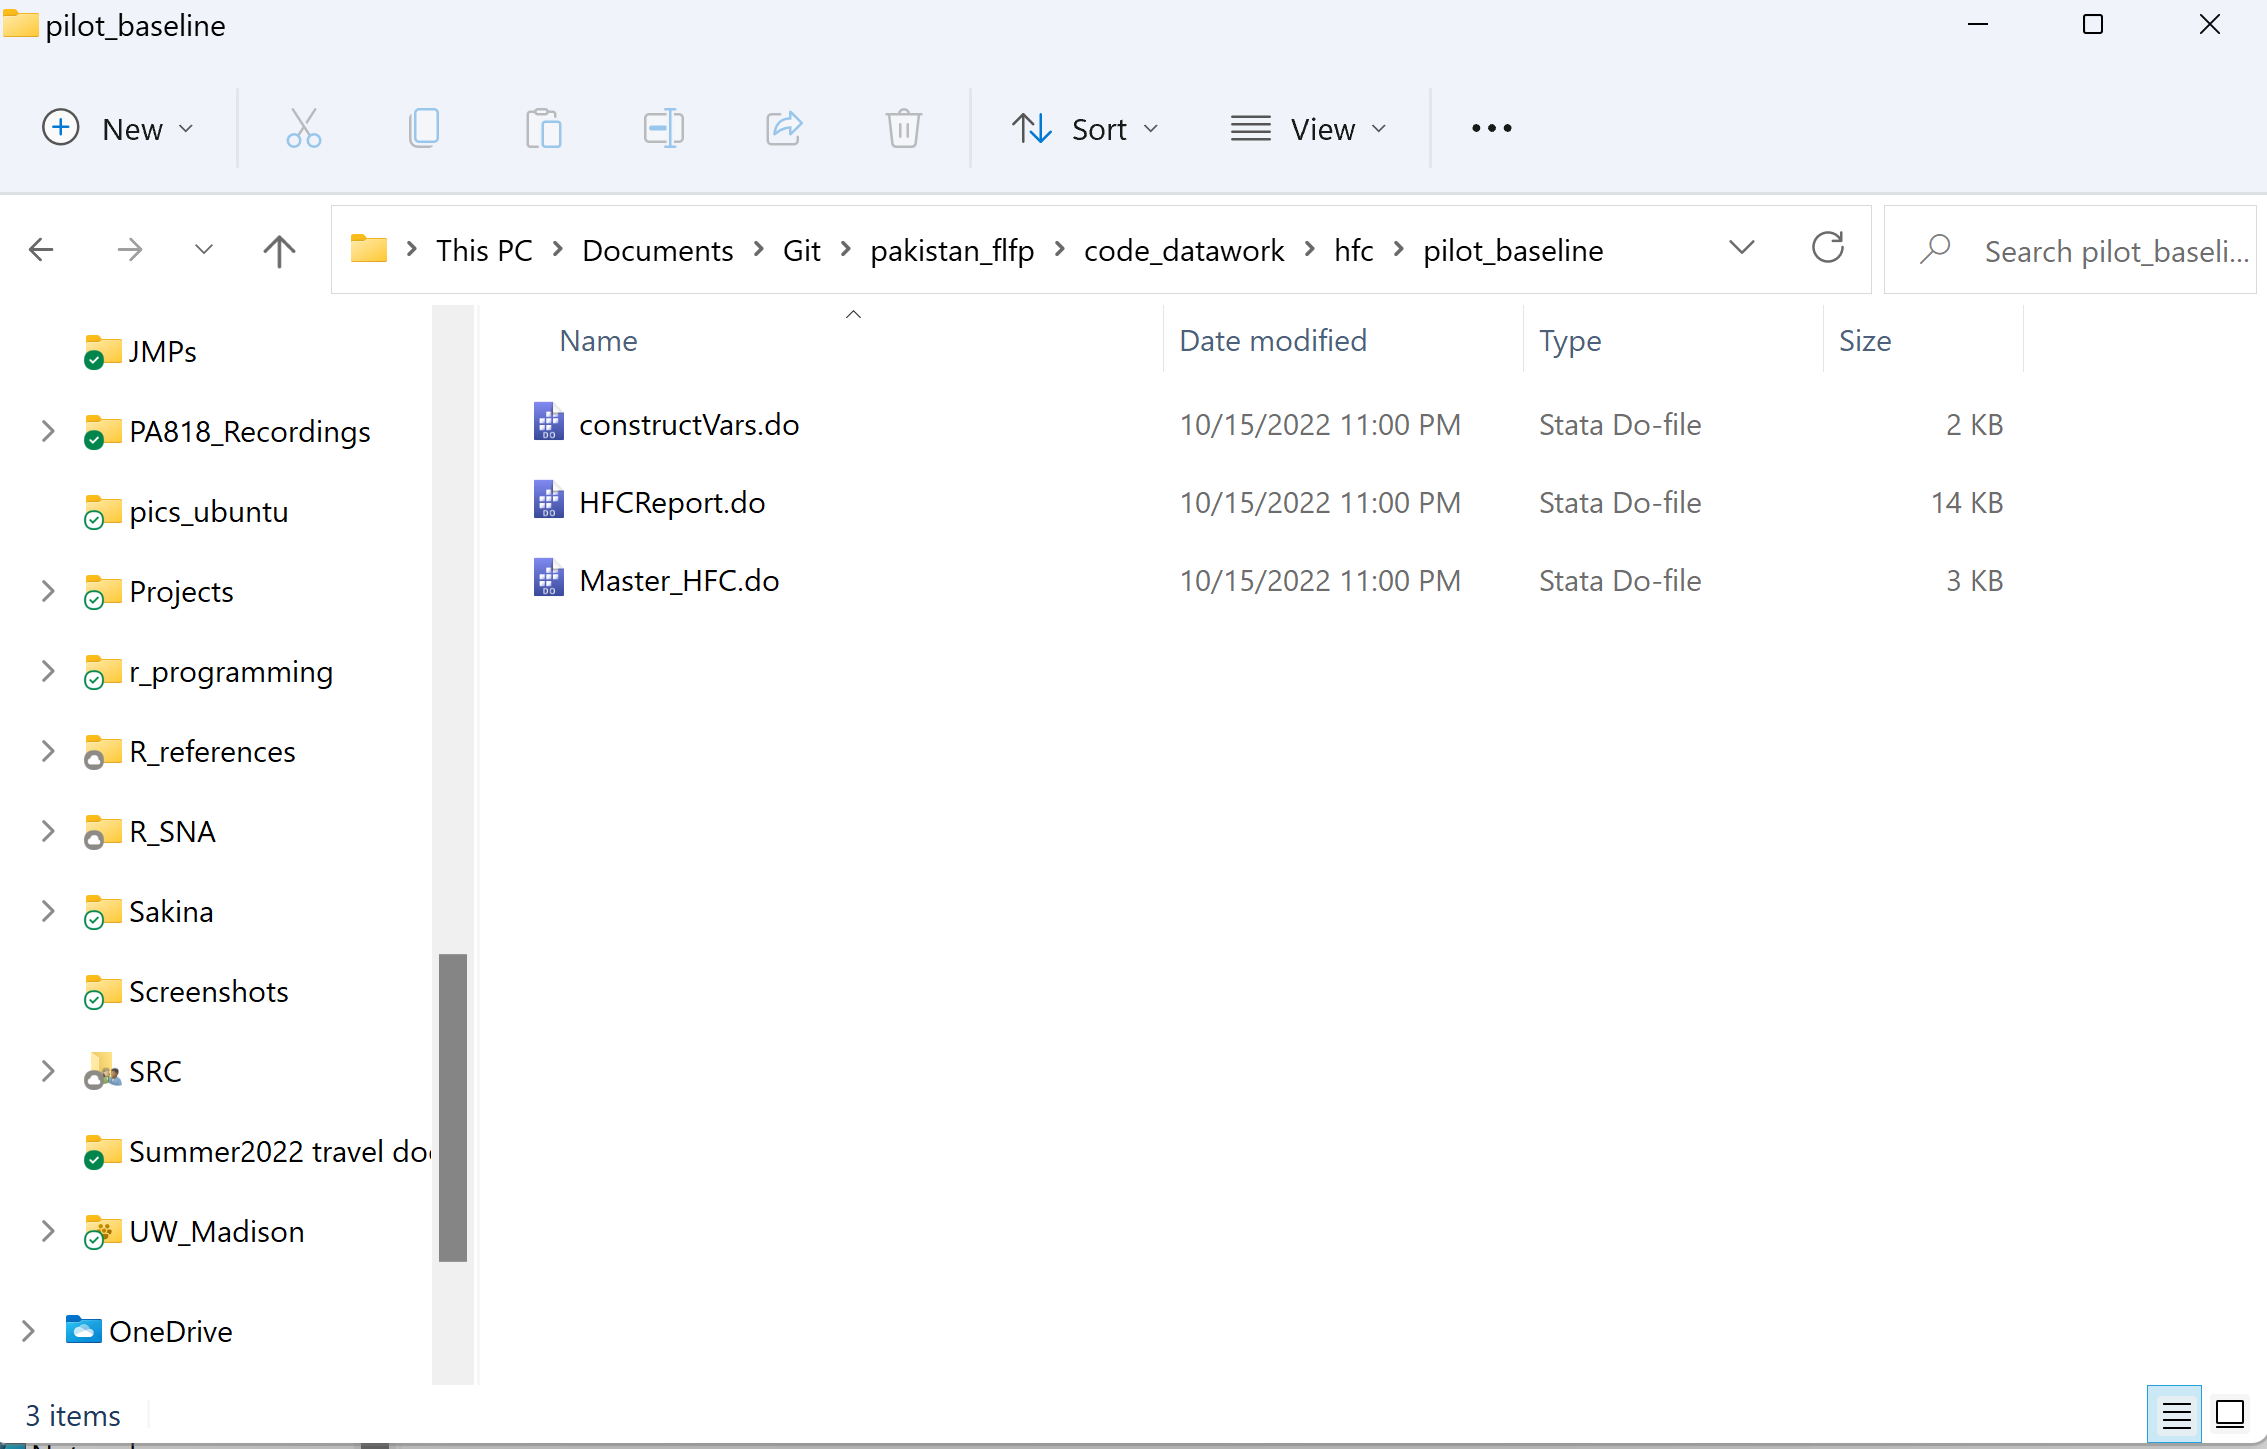
\includegraphics[width=0.7\linewidth]{example_folder}
	\label{fig:examplefolder}
\end{figure}
	

\subsection{Do-files Executable by All Your Team Members}

It's very important that your code is executable by your team members. \\ 

For this to be possible, they have to have proper access to input (i.e. data) and 
code. \\

One way to make your code executable by others is to have a "housekeeping" section as the following.
This one is from a project I'm working on with Zunia. \\ 

Notice that I have the following sections:
\begin{enumerate}
	\item User identification
	\item File directories
	\item Sections
	\item User-written commands
\end{enumerate}

\textbf{User identification} identifies your device and set folder paths to the folders shared by all the team members. \\

\textbf{File directories} make it clear where things are. \\

\textbf{Sections} provide a map for this current do file. \\

\textbf{User-written commands} make sure that everyone has all the necessary commands installed to run your code.

\newpage
\begin{stlog}{\smallskip}
***************
* Housekeeping 
***************
{\smallskip}
clear all
set more off
set mem 100m
set graphics off
{\smallskip}
{\smallskip}
* User identification
if c(username) == "sakina" {\lbr}
        global dropbox "C:\\Users\\sakina\\Dropbox\\Projects\\Pakistan_HiringCostsWomen"
        global git         "C:\\Users\\sakina\\Documents\\Git\\pakistan_flfp"
{\rbr}
{\smallskip}
if c(username) == "YourUserName" {\lbr}
        global dropbox "YourPathToYourDropboxFolder"
        global git         "YourPathToYourGitHubFolder"
{\rbr}
{\smallskip}
{\smallskip}
* File directories
global rawData          "$dropbox/Data/PrimaryData/rawData"
global modData          "$dropbox/Data/PrimaryData/modifiedData"
global dofiles          "$git/code_datawork"
global tables           "$git/output/tables/hfc/pilot_baseline"
global graphs           "$git/output/graphs/hfc/pilot_baseline"
global report           "$git/code_writings/HFCReports/pilot_baseline"
{\smallskip}
{\smallskip}
* Sections
global labeling         1
global cleanData        1
global constructVars  1
global analysis 1
{\smallskip}
        
* User-written commands
local download = 0 // Switch to 1 to user-written programs
if `download' {\lbr}
        ssc install texdoc, replace
        ssc install texsave, replace
        {\rbr}
\end{stlog}
\newpage
\section{Making Reproducible Tables}

We are going to use an example dataset that comes with Stata, called \textbf{nlswork.dta}. \\

If you want to know a bit about this dataset, simply

\begin{stlog}. webuse nlswork, clear
(National Longitudinal Survey of Young Women, 14-24 years old in 1968)
{\smallskip}
. notes
{\smallskip}
_dta:
  1.  Dataset is a subsample of the NLSY data.  Center for Human Resource Research. 1989. National Longitudinal Survey of Labor Market Experience, Young Women 14-24 years of
      age in 1968. Columbus, OH: Ohio State University Press.
{\smallskip}
\end{stlog}
We need to make one variable and change tha labels of two existing variables for our exercise. \\
\begin{stlog}gen black = (race == 2)
label var black "Black"
label var collgrad "College"
label var south "South"
\end{stlog}
\subsection{Making Tables with outreg2}

Suppose we are interested in understanding the relationships between wage and working hours (dependent variables), and education, race, and region in US in which respondents reside (independent variables). \\

We want to output the results into one table. \\

The easiest command for this purpose is probably \textit{outreg2}. \\

So we can run the following code. \\

\begin{stlog}{\smallskip}
{\smallskip}
reg ln_wage collgrad\#\#black i.year, r
estimates store reg1
        
reg ln_wage south\#\#black i.year, r
estimates store reg2
{\smallskip}
reg hours collgrad\#\#black i.year, r
estimates store reg3
        
reg hours south\#\#black i.year, r
estimates store reg4
{\smallskip}
{\smallskip}
outreg2 [reg1 reg2 reg3 reg4] using "$tables/regs_outreg2.tex", ///
        replace /// Replaces the existing file
        tex(frag) /// Creates a tex file without preembles
        label /// Use variable lables
        title("Correlation between Work, Race, Education, and Region") ///
        drop(i.year) /// Drop coefficients on the year FE
        dec(4) // Show estimates till 4th decimals
        
        
\end{stlog}

This command produces the following table. \\

\begin{table}[H]
	\centering
	\adjustbox{max width=\textwidth}{
	\begin{tabular}{lcccc}
\multicolumn{5}{c}{Correlation between Work, Race, Education, and Region} \\ \hline
 & (1) & (2) & (3) & (4) \\
 & reg1 & reg2 & reg3 & reg4 \\
VARIABLES & ln(wage/GNP deflator) & ln(wage/GNP deflator) & Usual hours worked & Usual hours worked \\ \hline
 &  &  &  &  \\
College = 1 & 0.3584*** &  & 2.2483*** &  \\
 & (0.0081) &  & (0.2085) &  \\
Black = 1 & -0.1291*** & 0.0241*** & 1.7113*** & 2.5414*** \\
 & (0.0060) & (0.0084) & (0.1245) & (0.1610) \\
0b.collgrad\#0b.black & 0.0000 &  & 0.0000 &  \\
 & (0.0000) &  & (0.0000) &  \\
0b.collgrad\#1o.black & 0.0000 &  & 0.0000 &  \\
 & (0.0000) &  & (0.0000) &  \\
1o.collgrad\#0b.black & 0.0000 &  & 0.0000 &  \\
 & (0.0000) &  & (0.0000) &  \\
1.collgrad\#1.black & 0.1497*** &  & -0.6171* &  \\
 & (0.0171) &  & (0.3343) &  \\
South = 1 &  & -0.1058*** &  & 2.3355*** \\
 &  & (0.0066) &  & (0.1480) \\
0b.south\#0b.black &  & 0.0000 &  & 0.0000 \\
 &  & (0.0000) &  & (0.0000) \\
0b.south\#1o.black &  & 0.0000 &  & 0.0000 \\
 &  & (0.0000) &  & (0.0000) \\
1o.south\#0b.black &  & 0.0000 &  & 0.0000 \\
 &  & (0.0000) &  & (0.0000) \\
1.south\#1.black &  & -0.2181*** &  & -2.8590*** \\
 &  & (0.0116) &  & (0.2321) \\
Constant & 1.4491*** & 1.5049*** & 36.7656*** & 36.2244*** \\
 & (0.0100) & (0.0103) & (0.2538) & (0.2589) \\
 &  &  &  &  \\
Observations & 28,534 & 28,526 & 28,467 & 28,460 \\
 R-squared & 0.1815 & 0.1292 & 0.0137 & 0.0164 \\ \hline
\multicolumn{5}{c}{ Robust standard errors in parentheses} \\
\multicolumn{5}{c}{ *** p$<$0.01, ** p$<$0.05, * p$<$0.1} \\
\end{tabular}

	}
\end{table}


This is fine for quick outputting, but it's very hard to read. \\

We also probably don't really need to show all estimates. \\

Let's say that we are only interested in the interacted terms for the purpose of this exercise. \\

The following table is much easier to read and looks more professional. \\

	\begin{table}[H]
		\centering
		\def\sym#1{\ifmmode^{#1}\else\(^{#1}\)\fi}
		\caption{Correlation between Work, Race, Education, and Region}
		\arrayrulecolor{black}
		\adjustbox{max width=\textwidth}{
		\begin{tabular}{lcc}
		\toprule
		& (1)  & (2)  \\
		& Wage & Work Hours \\
		\arrayrulecolor{black}\hline \\
		\textit{Panel A: Race and Education} & \multicolumn{1}{l}{} & \multicolumn{1}{l}{} \\
		College=1 $\times$ Black=1&       0.150***&      -0.617*  \\
                    &     [0.017]   &     [0.334]   \\
                    &               &               \\
Year FE             &         Yes   &         Yes   \\
Observations        &       28534   &       28467   \\
Dep. var. mean      &        1.67   &       36.56   \\
\hline \noalign{\smallskip}
 \\
		\textit{Panel B: Race and Region} & \multicolumn{1}{l}{} & \multicolumn{1}{l}{}  \\
		South=1 $\times$ Black=1&      -0.218***&      -2.859***\\
                    &     [0.012]   &     [0.232]   \\
                    &               &               \\
Year FE             &         Yes   &         Yes   \\
Observations        &       28526   &       28460   \\
Dep. var. mean      &        1.67   &       36.56   \\
\hline \noalign{\smallskip}
 \\
		\multicolumn{3}{p{.8\textwidth}}{\footnotesize
		\underline{Notes:} Robust standard errors
		in brackets.
		\sym{*} \(p<0.10\), \sym{**} \(p<0.05\), \sym{***} \(p<0.01\) \textit{Wage}
		is log-transformed and real, and \textit{work hours} indicates the number of hours
		usually worked. All data are from Stata's example data set \textit{nlswork.dta}. 
		The sample size of this data set is 28534.}
		\end{tabular}
		}
	\end{table}
 


Once we start thinking about more customization, we git the limitations of \textit{outreg2} quickly. \\

How can we make this table? \\
\newpage
\subsection{Making tables with estout and texdoc}

We can use \textit{estout} and \textit{texdoc} to achieve this. \\


\textbf{\textit{estout}} is a flexible command for outputting a table. \\

You can do all kinds of customization, although it can get pretty complicated. \\

I like to combined \textit{estout} and \textbf{\textit{texdoc}} to make my life a bit easier withouth compromizing on customizabiliy. \\


I won't really go deep into explaining \textit{texdoc}, because there is a very nice insturction on the web \href{http://repec.sowi.unibe.ch/stata/texdoc/getting-started.html}{by Ben Jann}. \\

I just note a couple of things.
\begin{itemize}
	\item The code that produces a tex file must be called from another do-file using the command \textit{textdoc do}.
	\item You also need to have \textit{stata.sty} in the same folder to complile the tex file.
\end{itemize}

Here is the code to do this. \\

\begin{stlog}{\smallskip}
****** Regression 1 : wage on educationXblack
{\smallskip}
        *** Estimate coefficients
        reg ln_wage collgrad\#\#black i.year, r
        eststo reg1_new // Storing the results in the way eststo can read.
                
        *** Year FE indicator
        estadd local yearFE "Yes", replace 
        
        *** Get the mean of dependent variables 
        sum ln_wage if e(sample), meanonly // if e(sample) calculates estimate using the regression sample
        local mean: di \%9.2f r(mean) // Setting the mean value at 2 decimals
        estadd local dvmean `mean', replace // Getting it ready to be added to the estout command later
        
        *** Add a blank row 
        estadd local blank " ", replace
        
{\smallskip}
****** Regression 2 : hours on educationXblack
{\smallskip}
        reg hours collgrad\#\#black i.year, r
        eststo reg2_new
        
        estadd local yearFE "Yes", replace 
        sum hours if e(sample), meanonly 
        local mean: di \%9.2f r(mean) 
        estadd local dvmean `mean', replace 
        estadd local blank " ", replace
        
{\smallskip}
{\smallskip}
****** Regression 3 : wage on southXblack
{\smallskip}
        reg ln_wage south\#\#black i.year, r
        eststo reg3_new
        
        estadd local yearFE "Yes", replace 
        sum ln_wage if e(sample), meanonly 
        local mean: di \%9.2f r(mean) 
        estadd local dvmean `mean', replace 
        estadd local blank " ", replace
{\smallskip}
{\smallskip}
****** Regression 4 : hours on southXblack              
{\smallskip}
        reg hours south\#\#black i.year, r
        eststo reg4_new
{\smallskip}
        estadd local yearFE "Yes", replace 
        sum hours if e(sample), meanonly 
        local mean: di \%9.2f r(mean) 
        estadd local dvmean `mean', replace 
        estadd local blank " ", replace
        
        
***** Ouput a table
{\smallskip}
        *** Panel A: educationXblack
        estout reg1_new reg2_new ///
                        using "$tables/regs_estout_panelA.tex", ///
                        style(tex) replace ///
                        keep(1.collgrad\#1.black) /// Keeping the estimate of interest.
                        interaction(" $\\times$ ") /// Specifying how the interaction is shown in the doc.
                        cells(b(star fmt(\%9.3f)) se(par([ ]) fmt(\%9.3f))) /// Setting how the point esitmate (b) and SE are shown. 
                        label nonumbers prehead() eqlabels(" ", none) /// Setting column titles
                        mgroups(, none) mlabels(, none) collabels(, none) /// Setting column titles
                        stats(blank yearFE N dvmean, fmt(0) /// Adding the stats and notes on FE 
                                  labels(" " "Year FE" "Observations" "Dep. var. mean")) /// Labeling the stats and notes on FE                  
                         postfoot(\\hline \\noalign{\lbr}\\smallskip{\rbr}) /// Writing out the lines at the bottom
        
        *** Panel B: southXblack
        estout reg3_new reg4_new ///
                        using "$tables/regs_estout_panelB.tex", ///
                        style(tex) replace ///
                        keep(1.south\#1.black) ///
                        interaction(" $\\times$ ") ///
                        cells(b(star fmt(\%9.3f)) se(par([ ]) fmt(\%9.3f))) ///
                        label nonumbers prehead() eqlabels(" ", none) ///
                        mgroups(, none) mlabels(, none) collabels(, none) ///
                        stats(blank yearFE N dvmean, fmt(0) ///
                                  labels(" " "Year FE" "Observations" ///
                                                 "Dep. var. mean")) ///
                         postfoot(\\hline \\noalign{\lbr}\\smallskip{\rbr})
                                         
\end{stlog}

After this part, you have to call the do file that writes out a whole tex file that companies \textit{Panel A} and \textit{Panel B} in a special way using the command, \textbf{\textit{texdoc do}} as the following: \\

\begin{verbatim}
texdoc do "\$dofiles/analysis/table\_regs\_estout.do"
\end{verbatim}


And this is what's inside of this do-file. \\


\begin{figure}[H]
	\centering
	\caption{Inside \textit{table\_regs\_estout.do}}
	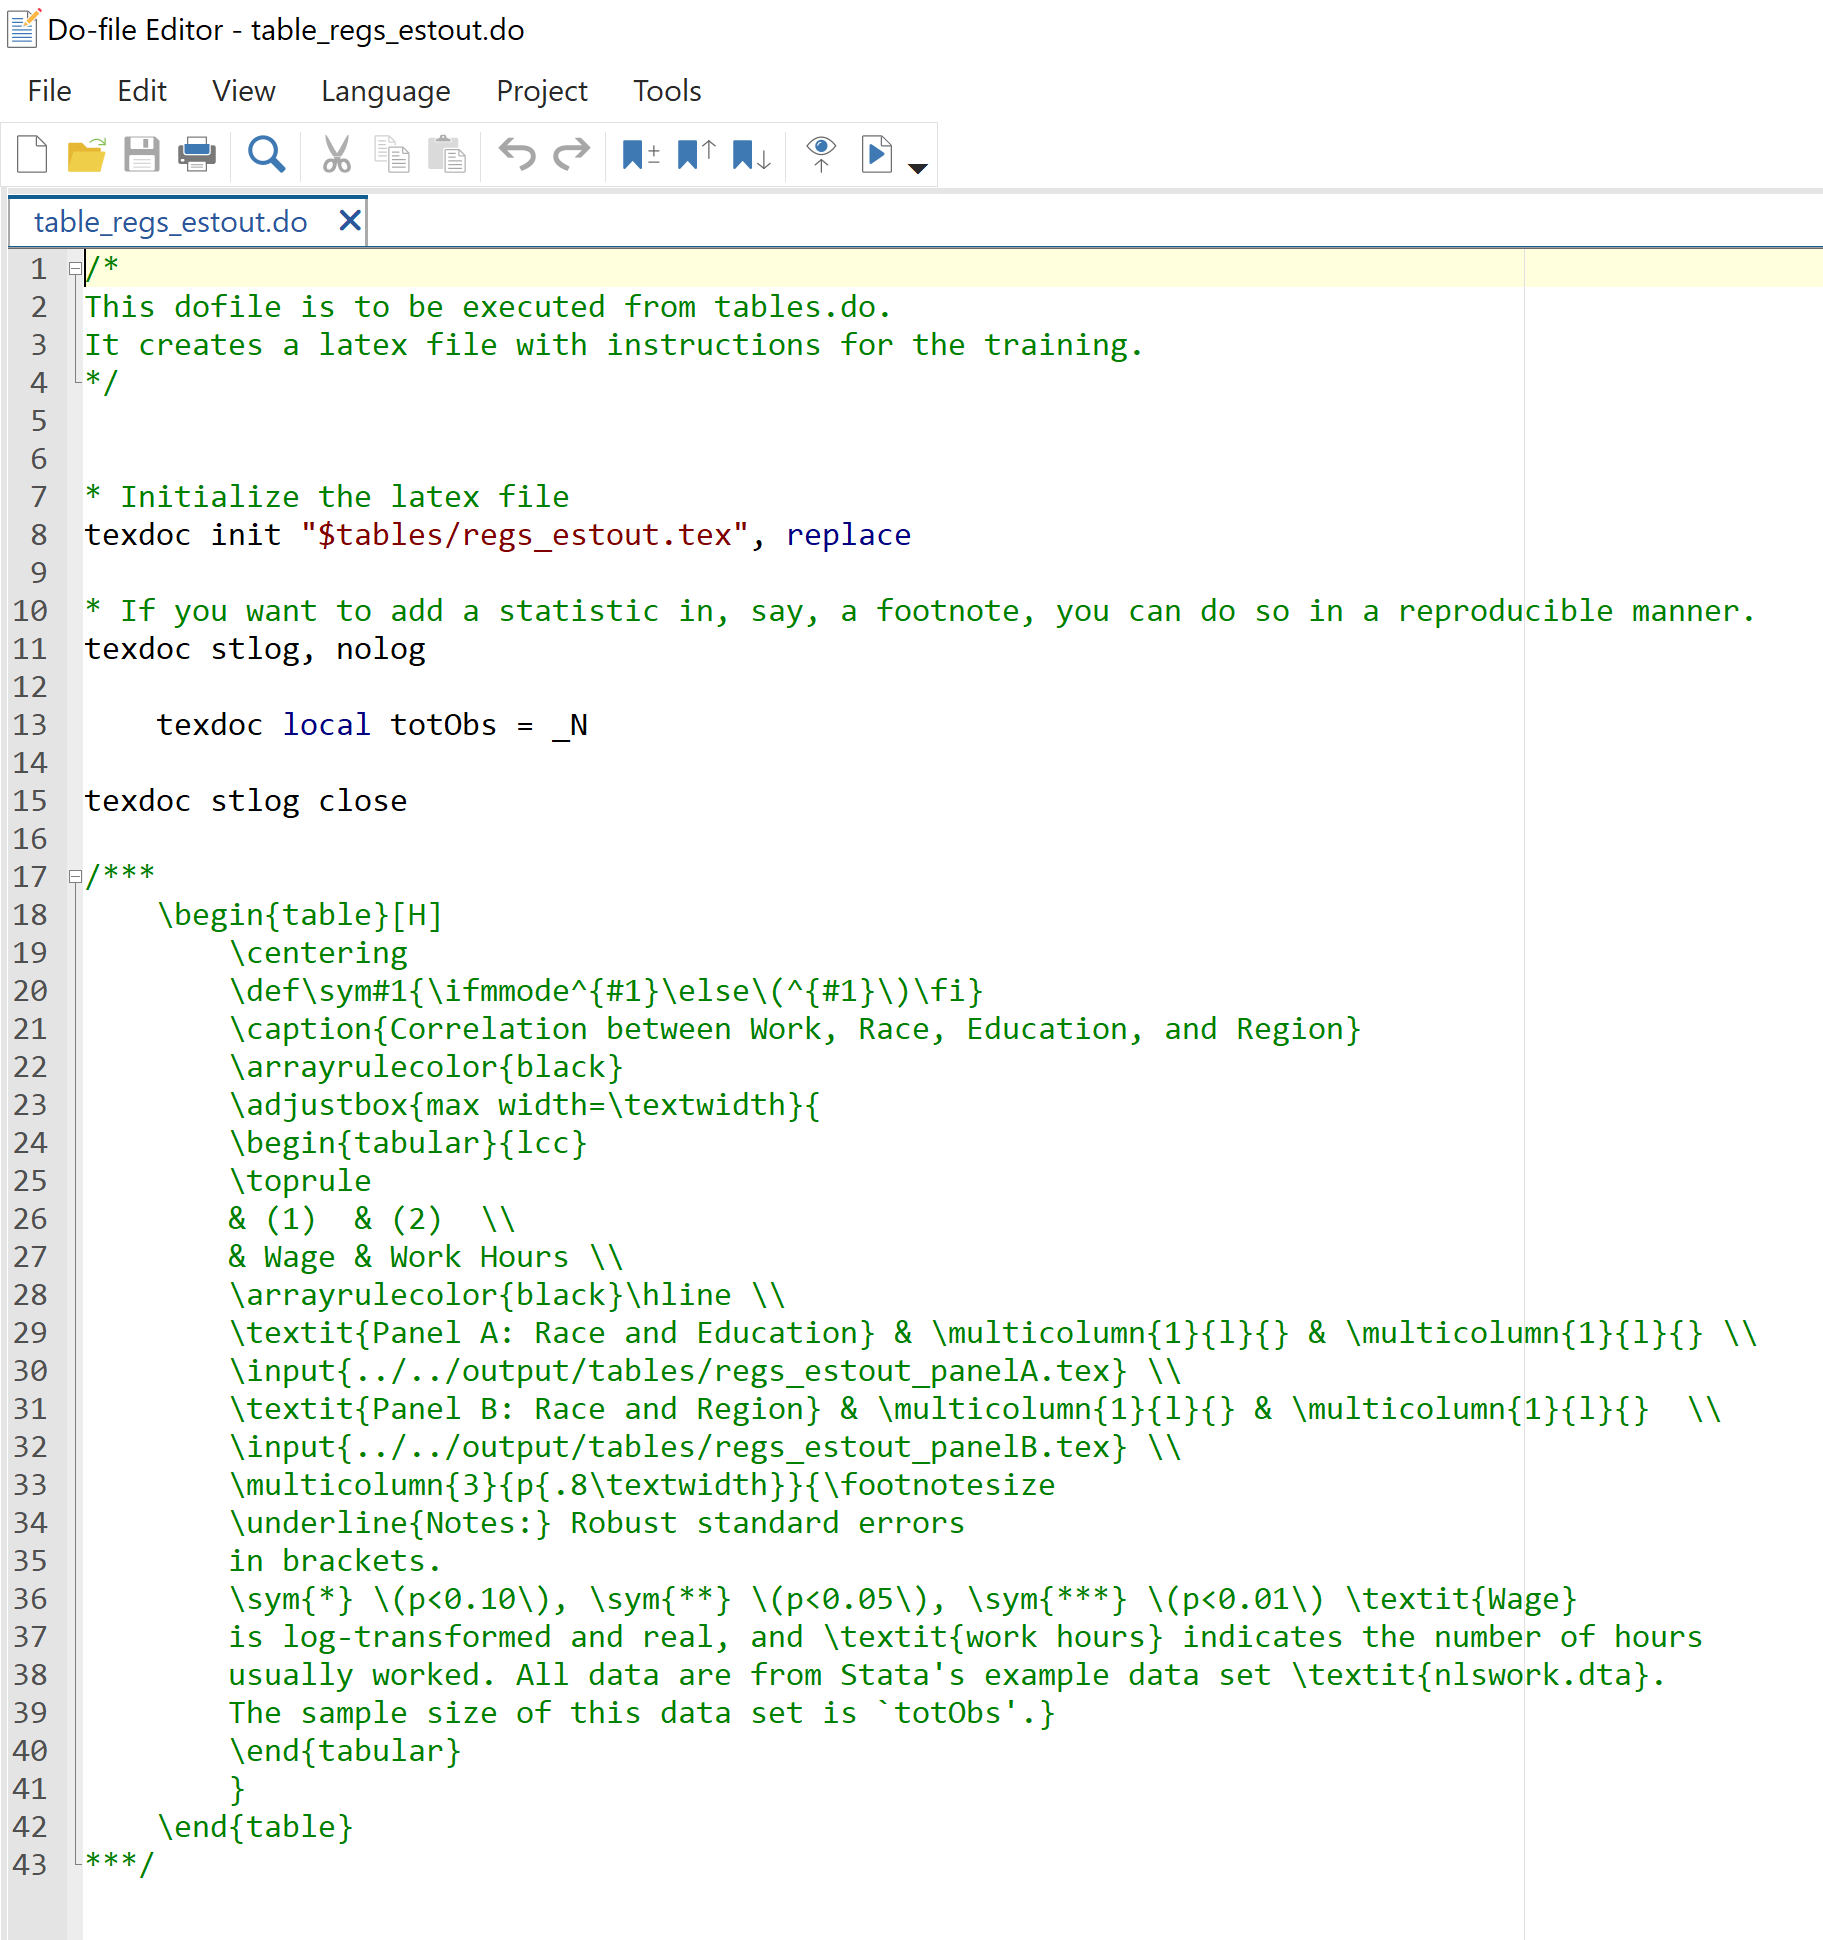
\includegraphics[width=\linewidth]{example_texdoc}
	\label{fig:exampletexdoc}
\end{figure}


This is the end of today's class. \\


Next time, we will cover how to use Git with Github. \\


Any questions and concerns?

\end{document}
